\chapter{Initial Evaluation}\label{C:init_eval}


\section{Current Experimental Setup}
The instrumentation as exists is assembled with an optical breadboard and XYZ+R stages with micrometre controls. A central stage holds the substrate with internally mounted thermocouple. Two manual focus cameras are positioned in profile and top down views, and the droplet is dispensed manually via a syringe mounted horizontally to a XYZ+R stage.
The current procedure is a manual process. The syringe tip is rotated above a marked point on the substrate, and hand emptied and refilled. This results in volume and positional variation between runs. This procedural variance is the focus of this project.

\section{Repeatability and Reliability}

Data taken from a series of five droplet runs was analysed to extract the variety in droplets and its effect on the measure temperature profile. 

\begin{figure}[h]
    \begin{center}
        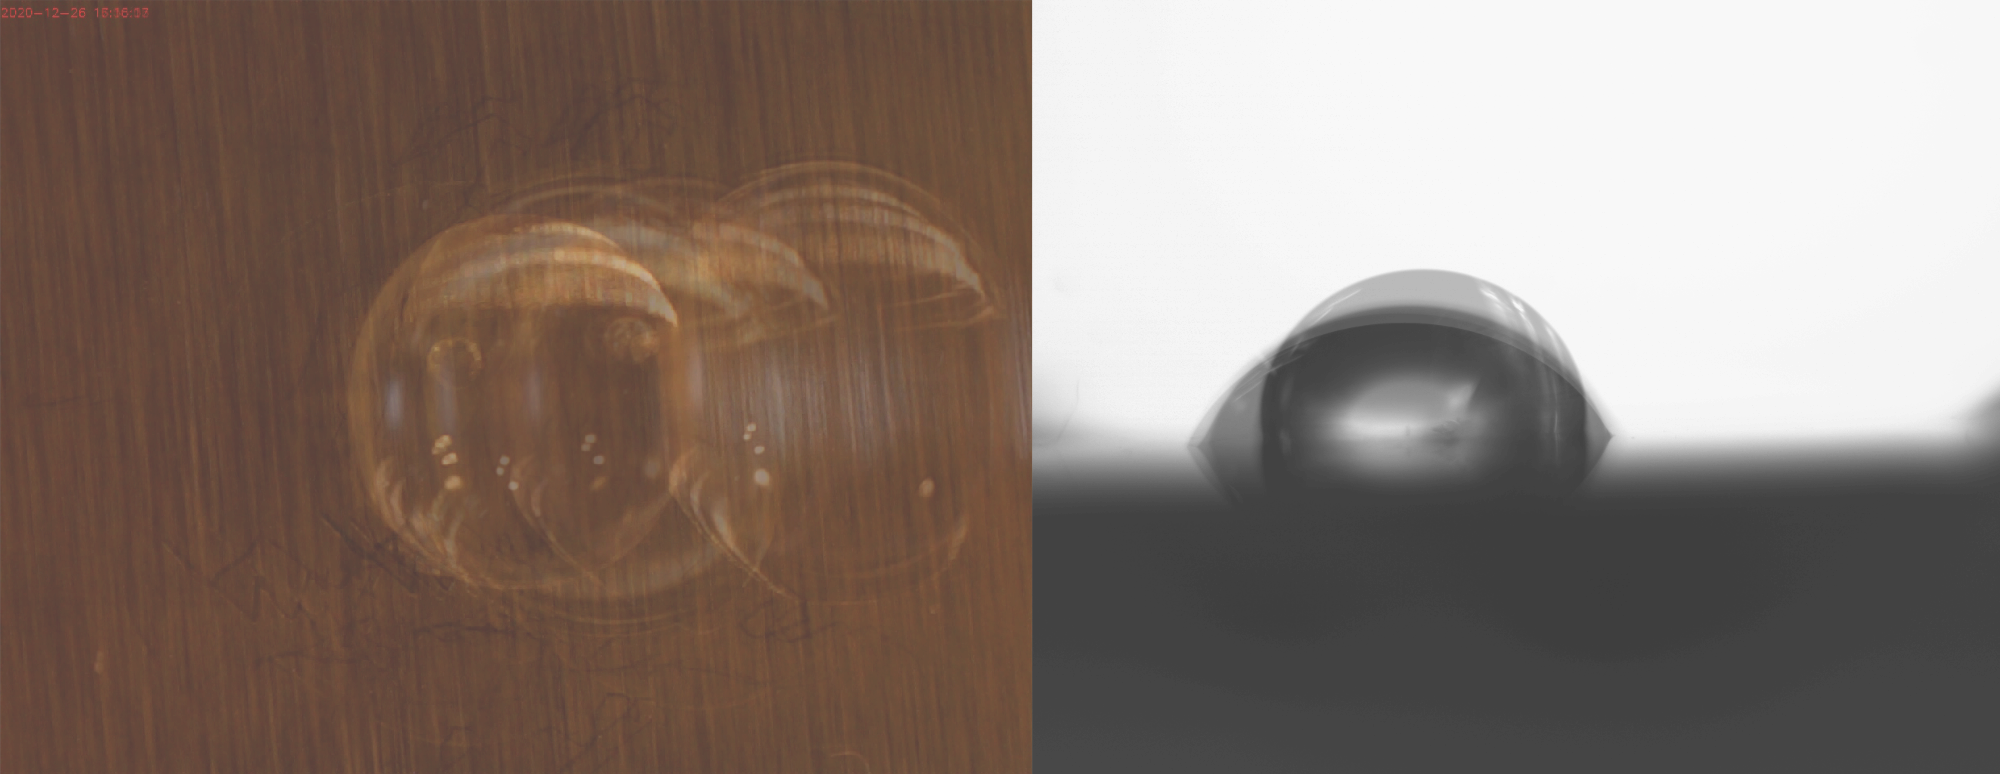
\includegraphics[width=.4\textwidth]{img/droplets_2018.png}
        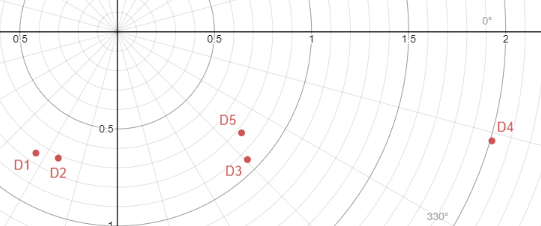
\includegraphics[width=.4\textwidth]{img/drop_pos_2018.png}

        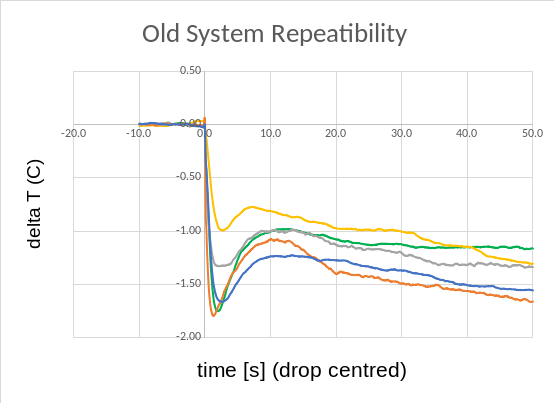
\includegraphics[width=.4\textwidth]{img/drop_temps_2018.png}
        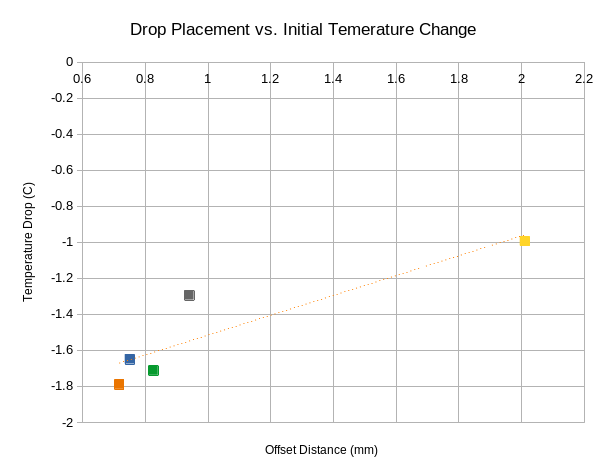
\includegraphics[width=.4\textwidth]{img/2018_pos_temp_trend.png}
    \end{center}
\end{figure}

\begin{table}[h]
    \centering
    \begin{tabular}{|l|l|l|}
    \hline
    \textit{\textbf{Droplet}} & \textit{Distance from Centre (mm)} & \textit{Estimated Volume (mm\textasciicircum{}2)} \\ \hline
    \cellcolor[HTML]{9698ED}1 & 0.7506                             & 16.55                                             \\ \hline
    \cellcolor[HTML]{E9AD3F}2 & 0.7164                             & 17.91                                             \\ \hline
    \cellcolor[HTML]{C0C0C0}3 & 0.9402                             & 17.89                                             \\ \hline
    \cellcolor[HTML]{FFFC9E}4 & 2.0104                             & 17.57                                             \\ \hline
    \cellcolor[HTML]{79CD5D}5 & 0.8258                             & 16.21                                             \\ \hline
    \end{tabular}
    \end{table}

\begin{table}[h]
    \centering
    \begin{tabular}{|l|l|l|}
    \hline
                   & \textit{Distance from Mark}          & \textit{Measured Temperature Drop} \\ \hline
    Min Pos Offset & 0.71mm                     &-1.7901$^{\circ}C$    \\ \hline
    Max Pos Offset &       2.01mm    &  -0.9944$^{\circ}C$    \\ \hline
                   & \textit{Volume}            & \textit{Contact Angle}          \\ \hline
    Shape Variance & $0.629mm^3$ & 25.894 degrees $\dagger$                \\ \hline
    \end{tabular}
    \caption{Variance in Setup}
    \subcaption*{$\dagger$This excluded an outlier of an almost spherical droplet with contact angles exceeding 95 degrees. This large variation is most likely due to inconsistency in surface chemisty from washing.}
    \end{table}


\section{Revised Approach}
The focus of the project is now twofold. Firstly on the automation of the process to allow for faster, pre-programmed runs to be carried out easier, and secondly to improve on the repeatability and reliability of the results by controlling the procedural factors of the experiment. 

An electronic pipette will be used to dispense a precise volume, and motorised stages will be used to provide preprogrammed, repeatable motion. The environmental factors however are not to be ignored, though controlling them is outside of the scope of this project. They will, however, be monitored, and this project will implement data collection of temperature, atmospheric pressure and humidity so these factors can be correlated to any remaining variation in data.  